% ============================================================
%  يُترجَم بـ XeLaTeX  (في Overleaf: Menu → Compiler → XeLaTeX)
%  الخط: Amiri (متوفر في Overleaf، أو حمّله من github.com/aliftype/amiri)
% ============================================================
\documentclass[12pt,a4paper]{article}
\usepackage[a4paper,margin=1.7cm,top=2.3cm,bottom=2.9cm,headheight=15pt,footskip=1.5cm]{geometry}
\usepackage{amsmath,amssymb}
\usepackage{icomma}
\usepackage[english,bidi=default,layout=lists]{babel}
\babelprovide[import,main]{arabic}
\babelfont{rm}[Scale=1.08]{Amiri}
\babelfont{sf}[Scale=1.08]{Amiri}
\usepackage[most]{tcolorbox}
\usepackage{tikz}
\usetikzlibrary{arrows.meta,calc,shadings}
\usepackage{array}
\usepackage{colortbl}
\usepackage{fancyhdr}
\usepackage{titlesec}
\usepackage{enumitem}
\usepackage{collcell}
\usepackage{needspace}
\usepackage{etoolbox}
\newcolumntype{C}{>{\collectcell\ar}c<{\endcollectcell}}
\pretocmd{\section}{\Needspace{15\baselineskip}}{}{}
\pretocmd{\subsection}{\Needspace{11\baselineskip}}{}{}

\definecolor{cDef}{HTML}{1F4E9C}
\definecolor{cThm}{HTML}{B3261E}
\definecolor{cRem}{HTML}{2E7D32}
\definecolor{cEx}{HTML}{C76B00}
\definecolor{cMeth}{HTML}{6A1B9A}
\definecolor{cSol}{HTML}{00695C}
\definecolor{cSec}{HTML}{1F3A68}

\titleformat{\section}{\Large\bfseries\color{cSec}}{\thesection.}{0.6em}{}[{\color{cSec!60}\titlerule[1pt]}]
\titleformat{\subsection}{\large\bfseries\color{cThm!85!black}}{\thesubsection.}{0.5em}{}
\titlespacing*{\section}{0pt}{14pt}{8pt}
\titlespacing*{\subsection}{0pt}{10pt}{5pt}
\setlength{\parindent}{0pt}
\setlength{\parskip}{4pt}
\setlist{itemsep=2pt,topsep=3pt}

\newtcolorbox{arbox}[3][]{enhanced,
  colback=#2!5,colframe=#2!80!black,arc=2mm,boxrule=0.8pt,
  left=6pt,right=6pt,top=8pt,bottom=5pt,
  fonttitle=\bfseries,coltitle=white,
  title={\foreignlanguage{arabic}{#3}},
  attach boxed title to top right={xshift=-5mm,yshift=-3mm},
  boxed title style={colback=#2!80!black,arc=1.5mm,boxrule=0pt},
  before upper={\selectlanguage{arabic}},
  before skip=8pt,after skip=8pt,breakable,#1}
\newenvironment{BOX}[2]{\begin{otherlanguage}{english}\begin{arbox}{#1}{#2}}{\end{arbox}\end{otherlanguage}}
\newenvironment{tarif}[1][تعريف]{\begin{BOX}{cDef}{#1}}{\end{BOX}}
\newenvironment{khassia}[1][خاصية]{\begin{BOX}{cThm}{#1}}{\end{BOX}}
\newenvironment{molahada}[1][ملاحظة]{\begin{BOX}{cRem}{#1}}{\end{BOX}}
\newenvironment{mithal}[1][مثال]{\begin{BOX}{cEx}{#1}}{\end{BOX}}
\newenvironment{tariqa}[1][طريقة]{\begin{BOX}{cMeth}{#1}}{\end{BOX}}

\newcounter{exo}
\newenvironment{tamrin}[1]{\stepcounter{exo}\begin{BOX}{cSec}{التمرين \theexo: #1}}{\end{BOX}}
\newenvironment{hal}{\Needspace{12\baselineskip}\begin{otherlanguage}{english}\begin{arbox}[breakable]{cSol}{حل التمرين \theexo}}{\end{arbox}\end{otherlanguage}}

\newenvironment{LTR}{\begin{otherlanguage}{english}}{\end{otherlanguage}}
\newcommand{\ar}[1]{\foreignlanguage{arabic}{#1}}

\renewcommand{\dots}{\mathinner{\ldotp\ldotp\ldotp}}
\renewcommand{\ldots}{\mathinner{\ldotp\ldotp\ldotp}}
\renewcommand{\cdots}{\mathinner{\cdotp\cdotp\cdotp}}
\newcommand{\N}{\mathbb{N}}
\newcommand{\Z}{\mathbb{Z}}
\newcommand{\D}{\mathbb{D}}
\newcommand{\Q}{\mathbb{Q}}
\newcommand{\R}{\mathbb{R}}
\newcommand{\pgcd}{\operatorname{PGCD}}
\newcommand{\ppcm}{\operatorname{PPCM}}

% \NLseg{a}{b}{[}{]} ; \NLright{a}{[} ; \NLleft{b}{]}  (interval on a number line)
\newcommand{\NLseg}[4]{\begin{LTR}\begin{tikzpicture}[baseline=-0.6ex]
 \draw[-{Stealth[length=2mm]},gray!70](0,0)--(3.4,0);
 \draw[line width=2pt,cThm!80!black](0.7,0)--(2.7,0);
 \node[cThm!80!black,font=\LARGE] at (0.7,0){$#3$};
 \node[cThm!80!black,font=\LARGE] at (2.7,0){$#4$};
 \node[below=3pt,font=\footnotesize] at (0.7,0){$#1$};
 \node[below=3pt,font=\footnotesize] at (2.7,0){$#2$};
\end{tikzpicture}\end{LTR}}
\newcommand{\NLright}[2]{\begin{LTR}\begin{tikzpicture}[baseline=-0.6ex]
 \draw[-{Stealth[length=2mm]},gray!70](0,0)--(3.4,0);
 \draw[line width=2pt,cThm!80!black](1.3,0)--(3.3,0);
 \node[cThm!80!black,font=\LARGE] at (1.3,0){$#2$};
 \node[below=3pt,font=\footnotesize] at (1.3,0){$#1$};
\end{tikzpicture}\end{LTR}}
\newcommand{\NLleft}[2]{\begin{LTR}\begin{tikzpicture}[baseline=-0.6ex]
 \draw[-{Stealth[length=2mm]},gray!70](0,0)--(3.4,0);
 \draw[line width=2pt,cThm!80!black](0.05,0)--(2.1,0);
 \node[cThm!80!black,font=\LARGE] at (2.1,0){$#2$};
 \node[below=3pt,font=\footnotesize] at (2.1,0){$#1$};
\end{tikzpicture}\end{LTR}}

% ---------- social-media icons (pure TikZ) ----------
\definecolor{cFB}{HTML}{1877F2}
\definecolor{cTG}{HTML}{229ED9}
\definecolor{cIG1}{HTML}{FEDA75}
\definecolor{cIG2}{HTML}{D62976}
\definecolor{cIG3}{HTML}{4F5BD5}
\newcommand{\fbicon}{\begin{LTR}\begin{tikzpicture}[baseline=-0.75ex,x=1em,y=1em]
 \fill[cFB] (0,0) circle (0.55);
 \node[white,inner sep=0,font=\usefont{TU}{lmss}{bx}{n}\small] at (0.04,-0.02) {f};
\end{tikzpicture}\end{LTR}}
\newcommand{\igicon}{\begin{LTR}
\begin{tikzpicture}[baseline=-0.75ex,x=1em,y=1em]
 \shade[lower left=cIG1,lower right=cIG2,upper left=cIG2,upper right=cIG3,rounded corners=0.28em] (-0.55,-0.55) rectangle (0.55,0.55);
 \draw[white,line width=0.09em,rounded corners=0.18em] (-0.36,-0.36) rectangle (0.36,0.36);
 \draw[white,line width=0.09em] (0,0) circle (0.17);
 \fill[white] (0.22,0.22) circle (0.05);
\end{tikzpicture}\end{LTR}}
\newcommand{\tgicon}{\begin{LTR}
\begin{tikzpicture}[baseline=-0.75ex,x=1em,y=1em]
 \fill[cTG] (0,0) circle (0.55);
 \fill[white] (-0.33,0.0) -- (0.32,0.27) -- (0.2,-0.3) -- (0.0,-0.15) -- (-0.08,-0.28) -- (-0.08,-0.08) -- cycle;
 \fill[cTG!70!black] (-0.08,-0.08) -- (0.25,0.2) -- (0.0,-0.15) -- (-0.08,-0.28) -- cycle;
\end{tikzpicture}\end{LTR}}
% page number: black box, white two-digit number, at the right of the social row
\newcommand{\PageBox}{\begin{LTR}\tikz[baseline=(p.base)]\node[fill=black,text=white,inner sep=2.5pt,minimum width=1.6em,minimum height=1.3em,font=\usefont{TU}{lmss}{bx}{n}\small](p){\ifnum\value{page}<10 0\fi\arabic{page}};\end{LTR}}
% visual left-to-right order: Telegram | Instagram | Facebook | page box
\newcommand{\SocialRow}{\begin{otherlanguage}{english}%
 \ar{\textbf{الأستاذ سوايسية هشام للرياضيات}}\ \tgicon\hfill
 \textbf{prof\_hicham\_math}\ \igicon\hfill
 \ar{\textbf{الأستاذ سوايسية هشام للرياضيات}}\ \fbicon\hspace{2.2em}\PageBox\end{otherlanguage}}

\pagestyle{fancy}
\fancyhf{}
\renewcommand{\headrulewidth}{0.6pt}
\renewcommand{\footrulewidth}{0.4pt}
% \SetHeader{right head: document title}{left head: level -- stream}
\newcommand{\SetHeader}[2]{%
 \fancyhead[C]{\parbox{\textwidth}{\ar{#1\hfill #2}}}%
 \fancyfoot[C]{\parbox{\textwidth}{\small\SocialRow}}}
\usepackage{tkz-tab}
\usepackage{multicol}
% variation / sign table (LTR)
\newenvironment{TAB}{\par\begin{center}\begin{LTR}\begin{tikzpicture}[scale=0.95,every node/.style={font=\small}]}{\end{tikzpicture}\end{LTR}\end{center}}
% grid + axes, clipped: \begin{GR}{xmin}{xmax}{ymin}{ymax}{unit cm}
\newenvironment{GR}[5]{\par\begin{center}\begin{LTR}\begin{tikzpicture}[x=#5cm,y=#5cm,font=\footnotesize]
 \draw[gray!25,very thin] (#1,#3) grid (#2,#4);
 \draw[-{Stealth[length=2mm]}] (#1,0)--(#2+0.3,0) node[below left]{$x$};
 \draw[-{Stealth[length=2mm]}] (0,#3)--(0,#4+0.3) node[below left]{$y$};
 \node[below left] at (0,0){$O$};
 \begin{scope}\clip (#1,#3) rectangle (#2,#4);}
{\end{scope}\end{tikzpicture}\end{LTR}\end{center}}
\newcommand{\Ticks}[2]{\foreach \t in {#1} \node[below,font=\scriptsize] at (\t,0){$\t$}; \foreach \t in {#2} \node[left,font=\scriptsize] at (0,\t){$\t$};}
\newcommand{\bx}[1]{\ensuremath{\colorbox{cDef!12}{$\displaystyle #1$}}}
\newcommand{\TwoCol}[4]{\par\begin{LTR}\noindent\begin{minipage}[t]{#1\textwidth}\selectlanguage{arabic}#2\end{minipage}\hfill\begin{minipage}[t]{#3\textwidth}\selectlanguage{arabic}#4\end{minipage}\end{LTR}\par}
\newcommand{\RL}[4]{\TwoCol{#3}{#4}{#1}{#2}}  % \RL{w1}{right content}{w2}{left content}
\newcommand{\ok}{$\textcolor{cRem}{\checkmark}$}
\newcommand{\limn}{\displaystyle\lim_{n\to+\infty}}
% sub-questions, each on its own line
\newenvironment{sq}{\begin{itemize}[leftmargin=2.4em,itemsep=3pt]}{\end{itemize}}
\newcommand{\qa}{\item[(أ)]}\newcommand{\qb}{\item[(ب)]}\newcommand{\qc}{\item[(جـ)]}\newcommand{\qd}{\item[(د)]}\newcommand{\qe}{\item[(هـ)]}
\newcommand{\pa}{\par\smallskip\textbf{(أ)} }\newcommand{\pb}{\par\smallskip\textbf{(ب)} }\newcommand{\pc}{\par\smallskip\textbf{(جـ)} }\newcommand{\pd}{\par\smallskip\textbf{(د)} }\newcommand{\pe}{\par\smallskip\textbf{(هـ)} }
\newcommand{\QQ}[1]{\par\smallskip\textbf{#1.} }
\newenvironment{tmr}{\stepcounter{exo}\begin{BOX}{cSec}{تمرين محلول \theexo}}{\end{BOX}}
\newcommand{\ABC}[3]{\\[2pt]\begin{tabular}{p{0.28\textwidth}p{0.28\textwidth}p{0.28\textwidth}}(جـ) \ #3 & (ب) \ #2 & (أ) \ #1\end{tabular}}
\pretocmd{\section}{\Needspace{24\baselineskip}}{}{}
\newtcbox{\bxtbox}{on line,colback=cDef!12,colframe=cDef!12,boxrule=0pt,arc=1pt,boxsep=0pt,left=2pt,right=2pt,top=1pt,bottom=1pt}
\newcommand{\bxt}[1]{\foreignlanguage{english}{\bxtbox{\ar{#1}}}}
\newcommand{\ua}{\ \mathrm{u.a}}
\newcommand{\dx}{\,\mathrm{d}x}
\newcommand{\dt}{\,\mathrm{d}t}
\SetHeader{\small\bfseries\color{cSec}ملخص: الدوال الأصلية والحساب التكاملي}{\small\color{cSec}السنة الثالثة ثانوي -- الشعب العلمية}
\begin{document}
\begin{LTR}
\begin{tcolorbox}[enhanced,colback=cSec,colframe=cSec,arc=3mm,halign=center,boxrule=0pt,top=12pt,bottom=12pt,before upper={\selectlanguage{arabic}}]
{\color{white}\fontsize{28}{34}\selectfont\bfseries الدوال الأصلية والحساب التكاملي}\\[8pt]
{\color{white}\large ملخص شامل مع أمثلة وتمارين محلولة خطوة بخطوة}\\[5pt]
{\color{white}\large السنة الثالثة ثانوي -- علوم تجريبية، رياضيات، تقني رياضي}
\end{tcolorbox}
\end{LTR}

\begin{BOX}{cSec}{محتوى الملخص}
\begin{multicols}{2}
\begin{enumerate}[label=\arabic*.]
\item الدوال الأصلية
\item جدول الدوال الأصلية المألوفة والعمليات
\item التكامل وخواصه
\item القيمة المتوسطة وحصر تكامل
\item التكامل بالتجزئة
\item حساب المساحات (والحجوم)
\item الدالة التكاملية والمتتاليات التكاملية
\item تمارين محلولة
\item خلاصة الطرائق
\end{enumerate}
\end{multicols}
\end{BOX}

%=====================================================
\section{الدوال الأصلية}
\begin{tarif}
$f$ دالة معرفة على مجال $I$. نقول إن الدالة $F$ \textbf{دالة أصلية} للدالة $f$ على $I$ إذا كانت $F$ قابلة للاشتقاق على $I$، ومن أجل كل $x$ من $I$:
\[ F'(x)=f(x) \]
\end{tarif}

\begin{khassia}
\begin{itemize}
\item كل دالة مستمرة على مجال $I$ تقبل دوالًا أصلية على $I$.
\item إذا كانت $F$ دالة أصلية للدالة $f$ على $I$ فإن الدوال الأصلية لـ $f$ على $I$ هي الدوال $x\mapsto F(x)+c$ حيث $c$ عدد حقيقي ثابت.
\item دالتان أصليتان لنفس الدالة على مجال تختلفان بثابت فقط.
\item من أجل $x_0$ من $I$ و $y_0$ عدد حقيقي، توجد \textbf{دالة أصلية وحيدة} $F$ للدالة $f$ على $I$ تحقق الشرط $F(x_0)=y_0$.
\end{itemize}
\end{khassia}

\begin{tariqa}[إثبات أن $F$ دالة أصلية لـ $f$]
نتحقق أن $F$ قابلة للاشتقاق على $I$، ثم نحسب $F'(x)$ ونبين أن $F'(x)=f(x)$ من أجل كل $x$ من $I$.\par
لإثبات أن $F$ و $G$ دالتان أصليتان لنفس الدالة: نبين أن $F'(x)=G'(x)$، أو أن $F(x)-G(x)$ ثابت.
\end{tariqa}

\begin{mithal}
\begin{itemize}
\item $F(x)=x\ln x-x$ على $]0;+\infty[$:
\[ F'(x)=\ln x+x\cdot\frac{1}{x}-1=\ln x \]
إذن \bxt{$F$ دالة أصلية للدالة $x\mapsto \ln x$ على $]0;+\infty[$}.
\item الدالتان $F(x)=x^{2}+3x+5$ و $G(x)=x^{2}+3x-7$: $F(x)-G(x)=12$ ثابت، إذن هما دالتان أصليتان لنفس الدالة $x\mapsto 2x+3$.
\end{itemize}
\end{mithal}

\begin{mithal}[دالة أصلية تأخذ قيمة معلومة]
$f(x)=3x^{2}+4x-2$ على $\R$. دوالها الأصلية: $F(x)=x^{3}+2x^{2}-2x+c$ حيث $c\in\R$.\par
الدالة الأصلية التي تحقق $F(1)=4$: $1+2-2+c=4$ أي $c=3$، إذن \bx{F(x)=x^{3}+2x^{2}-2x+3}.
\end{mithal}

%=====================================================
\section{جدول الدوال الأصلية المألوفة والعمليات}
\subsection{الدوال الأصلية المألوفة}
$c$ عدد حقيقي ثابت.
\begin{center}
\renewcommand{\arraystretch}{1.55}
\begin{tabular}{|>{\centering\arraybackslash}p{0.27\textwidth}|>{\centering\arraybackslash}p{0.3\textwidth}|>{\centering\arraybackslash}p{0.3\textwidth}|}\hline
\rowcolor{cSec!12}\textbf{المجال $I$} & \textbf{دالة أصلية $F$} & \textbf{الدالة $f$}\\\hline
$\R$ & $ax+c$ & $a$ (عدد حقيقي)\\\hline
$\R$ & $\dfrac{1}{n+1}x^{n+1}+c$ & $x^{n}$ \ ($n\in\N^{*}$)\\\hline
$]-\infty;0[$ أو $]0;+\infty[$ & $\dfrac{-1}{(n-1)x^{n-1}}+c$ & $\dfrac{1}{x^{n}}$ \ ($n\geqslant 2$)\\\hline
$]0;+\infty[$ & $2\sqrt{x}+c$ & $\dfrac{1}{\sqrt{x}}$\\\hline
$]0;+\infty[$ & $\ln x+c$ & $\dfrac{1}{x}$\\\hline
$\R$ & $e^{x}+c$ & $e^{x}$\\\hline
$\R$ & $\dfrac{1}{a}e^{ax+b}+c$ & $e^{ax+b}$ \ ($a\neq 0$)\\\hline
$\R$ & $-\cos x+c$ & $\sin x$\\\hline
$\R$ & $\sin x+c$ & $\cos x$\\\hline
$\R$ & $-\dfrac{1}{a}\cos(ax+b)+c$ & $\sin(ax+b)$ \ ($a\neq 0$)\\\hline
$\R$ & $\dfrac{1}{a}\sin(ax+b)+c$ & $\cos(ax+b)$ \ ($a\neq 0$)\\\hline
\end{tabular}
\end{center}

\subsection{الدوال الأصلية والعمليات}
$u$ دالة قابلة للاشتقاق على مجال $I$، و $n\in\N^{*}$.
\begin{center}
\renewcommand{\arraystretch}{1.55}
\begin{tabular}{|>{\centering\arraybackslash}p{0.3\textwidth}|>{\centering\arraybackslash}p{0.3\textwidth}|>{\centering\arraybackslash}p{0.27\textwidth}|}\hline
\rowcolor{cSec!12}\textbf{الشرط على $I$} & \textbf{دالة أصلية $F$} & \textbf{الدالة $f$}\\\hline
-- & $\dfrac{1}{n+1}u^{n+1}+c$ & $u'u^{n}$\\\hline
$u(x)\neq 0$ & $\dfrac{-1}{(n-1)u^{n-1}}+c$ & $\dfrac{u'}{u^{n}}$ \ ($n\geqslant 2$)\\\hline
$u(x)\neq 0$ & $-\dfrac{1}{u}+c$ & $\dfrac{u'}{u^{2}}$\\\hline
$u(x)>0$ & $2\sqrt{u}+c$ & $\dfrac{u'}{\sqrt{u}}$\\\hline
$u(x)>0$ & $\ln u+c$ & $\dfrac{u'}{u}$\\\hline
$u(x)\neq 0$ & $\ln|u|+c$ & $\dfrac{u'}{u}$\\\hline
-- & $e^{u}+c$ & $u'e^{u}$\\\hline
-- & $-\cos u+c$ & $u'\sin u$\\\hline
-- & $\sin u+c$ & $u'\cos u$\\\hline
\end{tabular}
\end{center}

\begin{tariqa}[تعيين دالة أصلية]
\begin{enumerate}
\item نلاحظ هل $f$ من أحد الأشكال: $u'u^{n}$، $\frac{u'}{u^{n}}$، $\frac{u'}{\sqrt{u}}$، $\frac{u'}{u}$، $u'e^{u}$؛ ونعين $u$ و $u'$.
\item إذا نقص معامل ثابت نكتب $f=k\times u'u^{n}$ (أو $k\times\frac{u'}{u}$ ...) ونخرج $k$.
\item نطبق الجدول، ولا ننسى الثابت $c$.
\end{enumerate}
\end{tariqa}

\begin{mithal}[الشكل $u'u^{n}$ و $\frac{u'}{u^{n}}$ و $\frac{u'}{\sqrt{u}}$]
\begin{enumerate}
\item $f(x)=(3x^{2}+2x)(x^{3}+x^{2}+7)^{2}$ على $\R$: $u(x)=x^{3}+x^{2}+7$، $u'(x)=3x^{2}+2x$، $n=2$:
\[ \bx{F(x)=\tfrac{1}{3}\left(x^{3}+x^{2}+7\right)^{3}+c} \]
\item $f(x)=(x+1)(2x^{2}+4x+1)^{2}$ على $\R$: $u(x)=2x^{2}+4x+1$، $u'(x)=4x+4=4(x+1)$، إذن $f=\frac{1}{4}u'u^{2}$:
\[ \bx{F(x)=\tfrac{1}{12}\left(2x^{2}+4x+1\right)^{3}+c} \]
\item $g(x)=\dfrac{2x}{(x^{2}+1)^{2}}$ على $\R$: من الشكل $\frac{u'}{u^{2}}$ مع $u(x)=x^{2}+1$: \bx{G(x)=-\dfrac{1}{x^{2}+1}+c}.
\item $h(x)=\dfrac{3x+1}{(3x^{2}+2x+7)^{3}}$ على $\R$: $u(x)=3x^{2}+2x+7$، $u'(x)=2(3x+1)$، إذن $h=\frac{1}{2}\cdot\frac{u'}{u^{3}}$:
\[ \bx{H(x)=\tfrac{1}{2}\times\frac{-1}{2u^{2}}+c=-\frac{1}{4\left(3x^{2}+2x+7\right)^{2}}+c} \]
\item $v(x)=\dfrac{5x}{\sqrt{x^{2}+1}}$ على $\R$: $v=\frac{5}{2}\cdot\frac{2x}{\sqrt{x^{2}+1}}=\frac{5}{2}\cdot\frac{u'}{\sqrt{u}}$، إذن \bx{V(x)=5\sqrt{x^{2}+1}+c}.
\end{enumerate}
\end{mithal}

\begin{mithal}[الشكل $\frac{u'}{u}$ و $u'e^{u}$]
\begin{enumerate}
\item $f(x)=\dfrac{1}{x+1}$ على $]-1;+\infty[$: $x+1>0$، إذن \bx{F(x)=\ln(x+1)+c}.
\item $f(x)=\dfrac{\cos x}{\sin x}$ على $]0;\pi[$: $\sin x>0$، إذن \bx{F(x)=\ln(\sin x)+c}.
\item $f(x)=\dfrac{x}{x^{2}-1}$ على $]1;+\infty[$: $f=\frac{1}{2}\cdot\frac{2x}{x^{2}-1}$، إذن \bx{F(x)=\tfrac{1}{2}\ln\left(x^{2}-1\right)+c}.
\item $f(x)=\dfrac{e^{x}}{e^{x}+1}$ على $\R$: \bx{F(x)=\ln\left(e^{x}+1\right)+c}.
\item $f(x)=\dfrac{1}{x\ln x}$ على $]1;+\infty[$: $f=\frac{(\ln x)'}{\ln x}$ و $\ln x>0$، إذن \bx{F(x)=\ln(\ln x)+c}.
\item $f(x)=\dfrac{\ln x}{x}$ على $]0;+\infty[$: $f=u'u$ مع $u=\ln x$، إذن \bx{F(x)=\tfrac{1}{2}(\ln x)^{2}+c}.
\item $f(x)=2xe^{x^{2}+3}$ على $\R$: \bx{F(x)=e^{x^{2}+3}+c}.
\item $f(x)=(x+1)e^{x^{2}+2x-5}$ على $\R$: $f=\frac{1}{2}(2x+2)e^{x^{2}+2x-5}$، إذن \bx{F(x)=\tfrac{1}{2}e^{x^{2}+2x-5}+c}.
\item $f(x)=e^{-3x+1}$ و $g(x)=\sin(2x+1)$ على $\R$: \bx{F(x)=-\tfrac{1}{3}e^{-3x+1}+c} و \bx{G(x)=-\tfrac{1}{2}\cos(2x+1)+c}.
\end{enumerate}
\end{mithal}

\begin{mithal}[كتابة $f$ على شكل مجموع ثم التكامل]
\begin{itemize}
\item $f(x)=\dfrac{2x+3}{x+1}$ على $]-1;+\infty[$: $f(x)=2+\dfrac{1}{x+1}$، إذن \bx{F(x)=2x+\ln(x+1)+c}.
\item $f(x)=\dfrac{1}{x-2}-\dfrac{1}{x+2}$ على $]2;+\infty[$: \bx{F(x)=\ln(x-2)-\ln(x+2)+c=\ln\dfrac{x-2}{x+2}+c}.
\end{itemize}
\end{mithal}

\begin{tariqa}[دالة أصلية من شكل معطى]
لتعيين $a$ و $b$ حتى تكون $F(x)=(ax+b)e^{x}$ دالة أصلية لـ $f$: نحسب $F'(x)$ ونطابقها مع $f(x)$ (مطابقة المعاملات).
\end{tariqa}

\begin{molahada}[المعادلتان $y'=f(x)$ و $y''=f(x)$]
\begin{itemize}
\item حلول $y'=f(x)$ هي الدوال $y=F(x)+c$ حيث $F$ دالة أصلية لـ $f$. مثال: $y'=\frac{1}{(x+1)^{2}}$ على $]-1;+\infty[$: $y=-\frac{1}{x+1}+c$.
\item حلول $y''=f(x)$ هي الدوال $y=G(x)+c_1x+c_2$ حيث $G$ دالة أصلية لدالة أصلية لـ $f$. مثال: $y''=4e^{2x}$: $y'=2e^{2x}+c_1$ ثم $y=e^{2x}+c_1x+c_2$.
\end{itemize}
\end{molahada}

%=====================================================
\section{التكامل وخواصه}
\begin{tarif}
$f$ دالة مستمرة على مجال $I$، و $a$، $b$ عددان من $I$، و $F$ دالة أصلية لـ $f$ على $I$. العدد الحقيقي $F(b)-F(a)$ يسمى \textbf{تكامل الدالة $f$ من $a$ إلى $b$}، ونكتب:
\[ \int_{a}^{b}f(x)\dx=\Big[F(x)\Big]_{a}^{b}=F(b)-F(a) \]
هذا العدد لا يتعلق باختيار الدالة الأصلية $F$، و $x$ متغير صامت: $\int_a^b f(x)\dx=\int_a^b f(t)\dt$.
\end{tarif}

\begin{mithal}
\begin{itemize}
\item $\displaystyle\int_{0}^{1}(3x^{2}+1)\dx=\Big[x^{3}+x\Big]_{0}^{1}=(1+1)-0=\bx{2}$
\item $\displaystyle\int_{1}^{e}\frac{1}{x}\dx=\Big[\ln x\Big]_{1}^{e}=\ln e-\ln 1=\bx{1}$
\item $\displaystyle\int_{-2}^{0}e^{2x+4}\dx=\Big[\tfrac{1}{2}e^{2x+4}\Big]_{-2}^{0}=\tfrac{1}{2}e^{4}-\tfrac{1}{2}e^{0}=\bx{\tfrac{1}{2}\left(e^{4}-1\right)}$
\item $\displaystyle\int_{0}^{\frac{\pi}{2}}\cos x\dx=\Big[\sin x\Big]_{0}^{\frac{\pi}{2}}=1-0=\bx{1}$
\item $\displaystyle\int_{0}^{1}\frac{x}{x^{2}+1}\dx=\Big[\tfrac{1}{2}\ln\left(x^{2}+1\right)\Big]_{0}^{1}=\bx{\tfrac{1}{2}\ln 2}$
\end{itemize}
\end{mithal}

\begin{khassia}[الخواص الجبرية]
$f$ و $g$ مستمرتان على $I$، و $a$، $b$، $c$ من $I$، و $\lambda\in\R$:
\begin{itemize}
\item $\displaystyle\int_a^a f(x)\dx=0$ \quad و \quad $\displaystyle\int_b^a f(x)\dx=-\int_a^b f(x)\dx$.
\item \textbf{علاقة شال:} $\displaystyle\int_a^c f(x)\dx+\int_c^b f(x)\dx=\int_a^b f(x)\dx$.
\item \textbf{الخطية:} $\displaystyle\int_a^b\big[f(x)+g(x)\big]\dx=\int_a^b f(x)\dx+\int_a^b g(x)\dx$ \quad و \quad $\displaystyle\int_a^b\lambda f(x)\dx=\lambda\int_a^b f(x)\dx$.
\end{itemize}
\end{khassia}

\begin{mithal}[علاقة شال مع القيمة المطلقة]
$|x|=-x$ على $[-1;0]$ و $|x|=x$ على $[0;2]$:
\[ \int_{-1}^{2}|x|\dx=\int_{-1}^{0}(-x)\dx+\int_{0}^{2}x\dx=\Big[-\tfrac{x^{2}}{2}\Big]_{-1}^{0}+\Big[\tfrac{x^{2}}{2}\Big]_{0}^{2}=\tfrac{1}{2}+2=\bx{\tfrac{5}{2}} \]
\end{mithal}

\begin{mithal}[استعمال الخطية]
$I=\displaystyle\int_0^1\frac{e^{x}}{e^{x}+1}\dx$ و $J=\displaystyle\int_0^1\frac{1}{e^{x}+1}\dx$.
\begin{itemize}
\item $I+J=\displaystyle\int_0^1\frac{e^{x}+1}{e^{x}+1}\dx=\int_0^1 1\dx=1$.
\item $I=\Big[\ln\left(e^{x}+1\right)\Big]_0^1=\ln(e+1)-\ln 2=\bx{\ln\dfrac{e+1}{2}}$، ومنه \bx{J=1-\ln\dfrac{e+1}{2}}.
\end{itemize}
\end{mithal}

\begin{khassia}[الإيجابية والمقارنة]
$a\leqslant b$ و $f$، $g$ مستمرتان على $[a;b]$:
\begin{itemize}
\item إذا كان $f(x)\geqslant 0$ من أجل كل $x$ من $[a;b]$ فإن $\displaystyle\int_a^b f(x)\dx\geqslant 0$.
\item إذا كان $f(x)\leqslant g(x)$ من أجل كل $x$ من $[a;b]$ فإن $\displaystyle\int_a^b f(x)\dx\leqslant\int_a^b g(x)\dx$.
\end{itemize}
\end{khassia}

\begin{molahada}
شرط $a\leqslant b$ أساسي: مثلا $\int_1^0 1\dx=-1<0$ رغم أن $1>0$.
\end{molahada}

\begin{khassia}[الزوجية والفردية]
$f$ مستمرة على $[-a;a]$ حيث $a>0$:
\begin{itemize}
\item إذا كانت $f$ \textbf{زوجية}: $\displaystyle\int_{-a}^{a}f(x)\dx=2\int_{0}^{a}f(x)\dx$. مثال: $\displaystyle\int_{-2}^{2}x^{2}\dx=2\Big[\tfrac{x^{3}}{3}\Big]_0^2=\tfrac{16}{3}$.
\item إذا كانت $f$ \textbf{فردية}: $\displaystyle\int_{-a}^{a}f(x)\dx=0$. مثال: $\displaystyle\int_{-1}^{1}x^{3}\cos x\dx=0$.
\end{itemize}
\end{khassia}

\RL{0.48}{%
\textbf{دالة زوجية:} المساحتان الملونتان متساويتان (تناظر بالنسبة لمحور التراتيب).}{0.48}{%
\textbf{دالة فردية:} المساحتان متساويتان والتكاملان متعاكسان (تناظر بالنسبة للمبدأ).}
\begin{LTR}
\noindent\begin{minipage}{0.48\textwidth}\centering
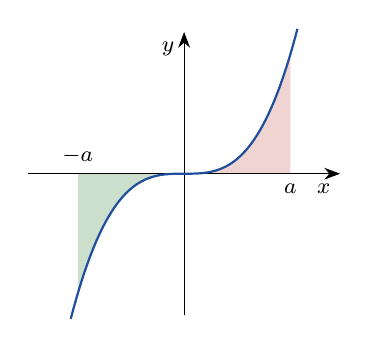
\begin{tikzpicture}[x=0.9cm,y=0.9cm,font=\footnotesize]
\fill[cRem!25,domain=-1.5:0,samples=60] (-1.5,0) -- plot(\x,{0.5*\x*\x*\x}) -- (0,0) -- cycle;
\fill[cThm!20,domain=0:1.5,samples=60] (0,0) -- plot(\x,{0.5*\x*\x*\x}) -- (1.5,0) -- cycle;
\draw[-{Stealth[length=2mm]}] (-2.2,0)--(2.2,0) node[below left]{$x$};
\draw[-{Stealth[length=2mm]}] (0,-2)--(0,2) node[below left]{$y$};
\draw[cDef,thick,domain=-1.6:1.6,samples=80] plot(\x,{0.5*\x*\x*\x});
\node[below] at (1.5,0){$a$}; \node[above] at (-1.5,0){$-a$};
\end{tikzpicture}
\end{minipage}\hfill
\begin{minipage}{0.48\textwidth}\centering
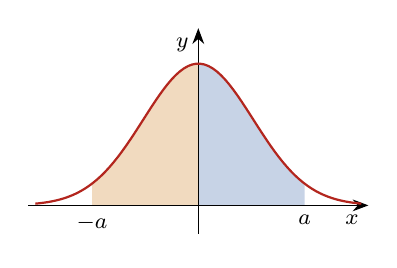
\begin{tikzpicture}[x=0.9cm,y=0.9cm,font=\footnotesize]
\fill[cEx!25,domain=-1.5:0,samples=60] (-1.5,0) -- plot(\x,{2*exp(-\x*\x/1.2)}) -- (0,0) -- cycle;
\fill[cDef!25,domain=0:1.5,samples=60] (0,0) -- plot(\x,{2*exp(-\x*\x/1.2)}) -- (1.5,0) -- cycle;
\draw[-{Stealth[length=2mm]}] (-2.4,0)--(2.4,0) node[below left]{$x$};
\draw[-{Stealth[length=2mm]}] (0,-0.4)--(0,2.5) node[below left]{$y$};
\draw[cThm,thick,domain=-2.3:2.3,samples=80] plot(\x,{2*exp(-\x*\x/1.2)});
\node[below] at (1.5,0){$a$}; \node[below] at (-1.5,0){$-a$};
\end{tikzpicture}
\end{minipage}
\end{LTR}

%=====================================================
\section{القيمة المتوسطة وحصر تكامل}
\begin{tarif}
$f$ مستمرة على $[a;b]$ حيث $a<b$. \textbf{القيمة المتوسطة} للدالة $f$ على $[a;b]$ هي العدد الحقيقي:
\[ m=\frac{1}{b-a}\int_a^b f(x)\dx \]
إذا كانت $f$ موجبة: مساحة الحيز تحت $(C_f)$ تساوي مساحة المستطيل الذي طوله $b-a$ وعرضه $m$.
\end{tarif}

\RL{0.5}{%
\begin{mithal}
القيمة المتوسطة للدالة $f(x)=x^{2}$ على $[0;3]$:
\[ m=\frac{1}{3-0}\int_0^3 x^{2}\dx=\frac{1}{3}\Big[\frac{x^{3}}{3}\Big]_0^3=\frac{1}{3}\times 9=\bx{3} \]
المساحة تحت المنحني ($9\ua$) تساوي مساحة المستطيل $3\times 3$.
\end{mithal}}{0.46}{%
\begin{LTR}\centering
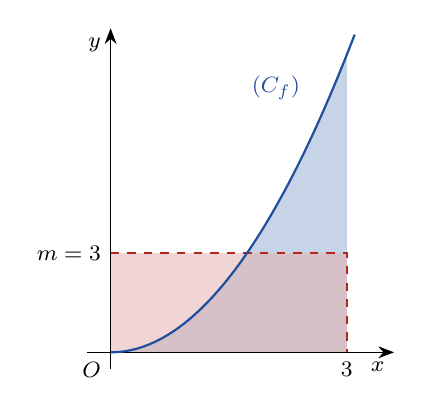
\begin{tikzpicture}[x=1cm,y=0.42cm,font=\footnotesize]
\fill[cDef!25,domain=0:3,samples=60] (0,0) -- plot(\x,{\x*\x}) -- (3,0) -- cycle;
\fill[cThm!35,opacity=0.55] (0,0) rectangle (3,3); \draw[cThm,thick,dashed] (0,3)--(3,3)--(3,0);
\draw[-{Stealth[length=2mm]}] (-0.3,0)--(3.6,0) node[below left]{$x$};
\draw[-{Stealth[length=2mm]}] (0,-0.5)--(0,9.8) node[below left]{$y$};
\draw[cDef,thick,domain=0:3.1,samples=60] plot(\x,{\x*\x});
\node[left] at (0,3){$m=3$}; \node[below] at (3,0){$3$}; \node[below left] at (0,0){$O$};
\node[cDef] at (2.1,8){$(C_f)$};
\end{tikzpicture}
\end{LTR}}

\begin{khassia}[حصر تكامل (متباينة المتوسط)]
إذا كان $a\leqslant b$ ومن أجل كل $x$ من $[a;b]$: $m\leqslant f(x)\leqslant M$، فإن:
\[ m(b-a)\leqslant\int_a^b f(x)\dx\leqslant M(b-a) \]
\end{khassia}

\begin{tariqa}[حصر تكامل]
\begin{enumerate}
\item نتأكد من استمرار $f$ على $[a;b]$ ومن أن $a\leqslant b$.
\item نحصر $f(x)$ من أجل $x\in[a;b]$ (باستعمال اتجاه التغير أو المتباينات).
\item نكامل طرفي الحصر من $a$ إلى $b$ (خاصية المقارنة).
\end{enumerate}
\end{tariqa}

\begin{mithal}
حصر $I=\displaystyle\int_0^1 e^{-x^{2}}\dx$: من أجل $x\in[0;1]$: $0\leqslant x^{2}\leqslant 1$، إذن $-1\leqslant -x^{2}\leqslant 0$، والدالة $\exp$ متزايدة، ومنه $e^{-1}\leqslant e^{-x^{2}}\leqslant 1$. بالمكاملة على $[0;1]$ (طوله $1$):
\[ \bx{\frac{1}{e}\leqslant I\leqslant 1} \]
\end{mithal}

%=====================================================
\section{التكامل بالتجزئة}
\begin{khassia}
$u$ و $v$ دالتان قابلتان للاشتقاق على مجال $I$ ومشتقتاهما $u'$ و $v'$ مستمرتان على $I$. من أجل كل $a$ و $b$ من $I$:
\[ \int_a^b u(x)v'(x)\dx=\Big[u(x)v(x)\Big]_a^b-\int_a^b u'(x)v(x)\dx \]
\end{khassia}

\begin{tariqa}[خطوات التكامل بالتجزئة]
\begin{enumerate}
\item نكتب $f(x)=u(x)\times v'(x)$: نختار $v'$ بحيث نعرف دالتها الأصلية $v$.
\item نحسب $u'$ و $v$، ثم نطبق القاعدة.
\item \textbf{أولوية اختيار $u$:} الدالة اللوغاريتمية، ثم كثير الحدود، ثم الدالة الأسية، ثم الدوال المثلثية.
\end{enumerate}
فإذا كانت $f(x)$ جداء كثير حدود في $e^{x}$ نضع $u(x)$ كثير الحدود؛ وإذا ظهر $\ln x$ نضع $u(x)=\ln x$.
\end{tariqa}

\begin{mithal}
\begin{enumerate}
\item $I=\displaystyle\int_0^1 xe^{x}\dx$: نضع $u(x)=x$، $v'(x)=e^{x}$ فيكون $u'(x)=1$، $v(x)=e^{x}$:
\[ I=\Big[xe^{x}\Big]_0^1-\int_0^1 e^{x}\dx=e-\Big[e^{x}\Big]_0^1=e-(e-1)=\bx{1} \]
\item $J=\displaystyle\int_1^e \ln x\dx$: نضع $u(x)=\ln x$، $v'(x)=1$ فيكون $u'(x)=\frac{1}{x}$، $v(x)=x$:
\[ J=\Big[x\ln x\Big]_1^e-\int_1^e 1\dx=e-(e-1)=\bx{1} \]
\item $K=\displaystyle\int_1^e x\ln x\dx$: نضع $u(x)=\ln x$، $v'(x)=x$ فيكون $u'(x)=\frac{1}{x}$، $v(x)=\frac{x^{2}}{2}$:
\[ K=\Big[\tfrac{x^{2}}{2}\ln x\Big]_1^e-\int_1^e\frac{x}{2}\dx=\frac{e^{2}}{2}-\Big[\frac{x^{2}}{4}\Big]_1^e=\frac{e^{2}}{2}-\frac{e^{2}-1}{4}=\bx{\frac{e^{2}+1}{4}} \]
\item $L=\displaystyle\int_0^{\pi}x\sin x\dx$: نضع $u(x)=x$، $v'(x)=\sin x$ فيكون $v(x)=-\cos x$:
\[ L=\Big[-x\cos x\Big]_0^{\pi}+\int_0^{\pi}\cos x\dx=\pi+\Big[\sin x\Big]_0^{\pi}=\bx{\pi} \]
\end{enumerate}
\end{mithal}

\begin{mithal}[تجزئة مرتين]
$M=\displaystyle\int_0^1 x^{2}e^{x}\dx$: نضع $u=x^{2}$، $v'=e^{x}$: $M=\Big[x^{2}e^{x}\Big]_0^1-2\displaystyle\int_0^1 xe^{x}\dx=e-2\times 1$، إذن \bx{M=e-2} (استعملنا $I=1$ من المثال السابق).
\end{mithal}

%=====================================================
\section{حساب المساحات (والحجوم)}
\begin{tarif}[وحدة المساحة]
في معلم متعامد $(O;\vec i,\vec j)$، \textbf{وحدة المساحة} $(\mathrm{u.a})$ هي مساحة المستطيل الذي بعداه $\|\vec i\|$ و $\|\vec j\|$.\par
مثلا: إذا كان $\|\vec i\|=2\,\mathrm{cm}$ و $\|\vec j\|=1\,\mathrm{cm}$ فإن $1\ua=2\,\mathrm{cm}^{2}$؛ وإذا كان $\|\vec i\|=\|\vec j\|=2\,\mathrm{cm}$ فإن $1\ua=4\,\mathrm{cm}^{2}$.
\end{tarif}

\begin{khassia}[المساحة بين منحنٍ ومحور الفواصل]
$f$ مستمرة على $[a;b]$ ($a<b$). مساحة الحيز $\mathcal{D}$ المحدد بـ $(C_f)$ ومحور الفواصل والمستقيمين $x=a$ و $x=b$:
\begin{itemize}
\item إذا كانت $f\geqslant 0$ على $[a;b]$: $\mathcal{A}=\displaystyle\int_a^b f(x)\dx\ua$.
\item إذا كانت $f\leqslant 0$ على $[a;b]$: $\mathcal{A}=-\displaystyle\int_a^b f(x)\dx\ua$.
\item إذا تغيرت إشارة $f$ عند $c$: نجزئ بعلاقة شال؛ وفي كل الحالات $\mathcal{A}=\displaystyle\int_a^b |f(x)|\dx\ua$.
\end{itemize}
\end{khassia}

\begin{tariqa}[حساب مساحة]
\begin{enumerate}
\item نرسم المنحنيات ونلون الحيز.
\item ندرس إشارة $f(x)$ (أو $f(x)-g(x)$) على $[a;b]$ في جدول.
\item نكتب المساحة $\int_a^b|\ldots|$ بالإشارة الصحيحة، ثم نحسب بالـ $\mathrm{u.a}$ ثم بالـ $\mathrm{cm}^{2}$.
\end{enumerate}
\end{tariqa}

\begin{mithal}[$f$ موجبة]
$f(x)=-x^{2}+4x=x(4-x)$ على $[0;4]$:
\begin{TAB}
\tkzTabInit[lgt=2.2,espcl=4]{$x$ /0.8,$f(x)$ /0.8}{$0$,$4$}
\tkzTabLine{z,+,z}
\end{TAB}
$f(x)\geqslant 0$ على $[0;4]$، إذن:
\[ \mathcal{A}=\int_0^4\left(-x^{2}+4x\right)\dx=\Big[-\frac{x^{3}}{3}+2x^{2}\Big]_0^4=-\frac{64}{3}+32=\bx{\frac{32}{3}\ua} \]
\begin{GR}{-1}{5}{-1}{5}{0.75}
\fill[cDef!25,domain=0:4,samples=100] (0,0) -- plot(\x,{-\x*\x+4*\x}) -- (4,0) -- cycle;
\draw[cDef,thick,domain=-0.6:4.6,samples=100] plot(\x,{-\x*\x+4*\x});
\node at (2,1.6){$\mathcal{A}$};
\node[cDef] at (3.9,3.8){$(C_f)$};
\Ticks{1,2,3,4}{1,2,3,4}
\end{GR}
\end{mithal}

\begin{mithal}[$f$ تغير إشارتها]
$f(x)=x^{2}-1$ على $[0;2]$:
\begin{TAB}
\tkzTabInit[lgt=2.2,espcl=3]{$x$ /0.8,$f(x)$ /0.8}{$0$,$1$,$2$}
\tkzTabLine{,-,z,+,}
\end{TAB}
\[ \mathcal{A}=\int_0^2|f(x)|\dx=-\int_0^1\left(x^{2}-1\right)\dx+\int_1^2\left(x^{2}-1\right)\dx=\Big[x-\frac{x^{3}}{3}\Big]_0^1+\Big[\frac{x^{3}}{3}-x\Big]_1^2 \]
\[ \mathcal{A}=\mathcal{A}_1+\mathcal{A}_2=\frac{2}{3}+\frac{4}{3}=\bx{2\ua} \]
\begin{GR}{-1}{3}{-2}{4}{0.75}
\fill[cThm!20,domain=0:1,samples=100] (0,0) -- plot(\x,{\x*\x-1}) -- (1,0) -- cycle;
\fill[cDef!25,domain=1:2,samples=100] (1,0) -- plot(\x,{\x*\x-1}) -- (2,0) -- cycle;
\draw[cDef,thick,domain=-1:2.3,samples=100] plot(\x,{\x*\x-1});
\draw[dashed] (2,0)--(2,3);
\node at (0.45,-0.35){$\mathcal{A}_1$}; \node at (1.7,0.8){$\mathcal{A}_2$};
\node[cDef] at (2.6,3.4){$(C_f)$};
\Ticks{1,2}{1,2,3}
\end{GR}
\end{mithal}

\begin{khassia}[المساحة بين منحنيين]
$f$ و $g$ مستمرتان على $[a;b]$. مساحة الحيز المحدد بـ $(C_f)$ و $(C_g)$ والمستقيمين $x=a$ و $x=b$:
\[ \mathcal{A}=\int_a^b\big|f(x)-g(x)\big|\dx\ua \]
إذا كان $(C_f)$ فوق $(C_g)$ على $[a;b]$: $\mathcal{A}=\displaystyle\int_a^b\big[f(x)-g(x)\big]\dx\ua$. وتبقى صحيحة إذا كان $(C_g)$ مستقيمًا مقاربًا $(\Delta):y=\alpha x+\beta$.
\end{khassia}

\begin{mithal}[بين قطع مكافئ ومستقيم]
$f(x)=4-x^{2}$ و $g(x)=x+2$. نقطتا التقاطع: $4-x^{2}=x+2\iff x^{2}+x-2=0\iff x=-2$ أو $x=1$.\par
$f(x)-g(x)=-x^{2}-x+2=-(x+2)(x-1)$:
\begin{TAB}
\tkzTabInit[lgt=3,espcl=3.5]{$x$ /0.8,$f(x)-g(x)$ /0.8,\ar{الوضع النسبي} /1}{$-2$,$1$}
\tkzTabLine{z,+,z}
\tkzTabLine{,\text{\scriptsize\ar{$(C_f)$ فوق $(C_g)$}},}
\end{TAB}
\[ \mathcal{A}=\int_{-2}^{1}\left(-x^{2}-x+2\right)\dx=\Big[-\frac{x^{3}}{3}-\frac{x^{2}}{2}+2x\Big]_{-2}^{1}=\frac{7}{6}-\left(-\frac{10}{3}\right)=\bx{\frac{9}{2}\ua} \]
\begin{GR}{-3}{3}{-2}{5}{0.7}
\fill[cEx!25,domain=-2:1,samples=100] plot(\x,{4-\x*\x}) -- plot[domain=1:-2](\x,{\x+2}) -- cycle;
\draw[cDef,thick,domain=-2.6:2.6,samples=100] plot(\x,{4-\x*\x});
\draw[cThm,thick,domain=-3:2.8] plot(\x,{\x+2});
\node at (-0.4,2.4){$\mathcal{A}$};
\node[cDef] at (2.4,-1.4){$(C_f)$}; \node[cThm] at (2.2,4.6){$(C_g)$};
\Ticks{-2,-1,1,2}{1,2,3,4}
\end{GR}
\end{mithal}

\begin{mithal}[بين منحنٍ ومستقيمه المقارب، والنهاية]
$f(x)=x+1+e^{-x}$ على $\R$، و $(\Delta):y=x+1$ مقارب مائل عند $+\infty$. من أجل $\lambda>0$:
\begin{TAB}
\tkzTabInit[lgt=3,espcl=3.5]{$x$ /0.8,$f(x)-(x+1)$ /0.8,\ar{الوضع النسبي} /1}{$0$,$\lambda$}
\tkzTabLine{,+,}
\tkzTabLine{,\text{\scriptsize\ar{$(C_f)$ فوق $(\Delta)$}},}
\end{TAB}
\[ \mathcal{A}(\lambda)=\int_0^{\lambda}\big[f(x)-(x+1)\big]\dx=\int_0^{\lambda}e^{-x}\dx=\Big[-e^{-x}\Big]_0^{\lambda}=\bx{1-e^{-\lambda}\ua} \]
$\displaystyle\lim_{\lambda\to+\infty}\mathcal{A}(\lambda)=1$. إذا كان $\|\vec i\|=\|\vec j\|=2\,\mathrm{cm}$: $\mathcal{A}(\lambda)=4\left(1-e^{-\lambda}\right)\,\mathrm{cm}^{2}$.
\begin{GR}{-1}{4}{-1}{5}{0.7}
\fill[cRem!25,domain=0:3,samples=100] plot(\x,{\x+1+exp(-\x)}) -- plot[domain=3:0](\x,{\x+1}) -- cycle;
\draw[cThm,thick,domain=-1:4] plot(\x,{\x+1});
\draw[cDef,thick,domain=-0.9:4,samples=100] plot(\x,{\x+1+exp(-\x)});
\draw[dashed] (3,0)--(3,4);
\node[below] at (3,0){$\lambda$};
\node at (0.9,2.25){$\mathcal{A}$};
\node[cDef] at (0.6,3.6){$(C_f)$}; \node[cThm] at (3.4,3.4){$(\Delta)$};
\Ticks{1,2}{1,2,3,4}
\end{GR}
\end{mithal}

\begin{khassia}[حجم مجسم دوراني -- شعبة رياضيات أساسًا]
\begin{itemize}
\item إذا كانت $S(z)$ مساحة مقطع مجسم بمستوٍ يعامد المحور عند الراقم $z$ حيث $a\leqslant z\leqslant b$: $V=\displaystyle\int_a^b S(z)\,\mathrm{d}z$ (وحدة الحجوم).
\item دوران $(C_f)$ حول محور الفواصل على $[a;b]$ يولد مجسما حجمه $V=\displaystyle\int_a^b\pi\big[f(x)\big]^{2}\dx$.
\end{itemize}
مثال: $f(x)=\sqrt{x}$ على $[0;4]$: $V=\pi\displaystyle\int_0^4 x\dx=\pi\Big[\frac{x^{2}}{2}\Big]_0^4=\bx{8\pi}$ وحدة حجوم.
\end{khassia}

%=====================================================
\section{الدالة التكاملية والمتتاليات التكاملية}
\begin{khassia}[الدالة $F(x)=\int_a^x f(t)\dt$]
$f$ مستمرة على مجال $I$ و $a\in I$. الدالة $F:x\mapsto\displaystyle\int_a^x f(t)\dt$ هي \textbf{الدالة الأصلية الوحيدة} للدالة $f$ على $I$ التي تنعدم عند $a$:
\[ F'(x)=f(x)\qquad\text{و}\qquad F(a)=0 \]
\end{khassia}

\begin{mithal}
\begin{itemize}
\item $F(x)=\displaystyle\int_1^x\ln t\dt$ على $]0;+\infty[$: بالتجزئة ($u=\ln t$، $v'=1$): $F(x)=\Big[t\ln t\Big]_1^x-\displaystyle\int_1^x 1\dt$، إذن \bx{F(x)=x\ln x-x+1}.
\item $G(x)=\displaystyle\int_0^x e^{-t^{2}}\dt$: لا نعرف عبارتها، لكن $G'(x)=e^{-x^{2}}>0$، إذن \bxt{$G$ متزايدة تمامًا على $\R$}، و $G(0)=0$.
\item (رياضيات) إذا كانت $u$ قابلة للاشتقاق:
\[ \left(\int_a^{u(x)}f(t)\dt\right)'=u'(x)\,f\big(u(x)\big) \]
مثلا $H(x)=\displaystyle\int_0^{x^{2}}e^{-t^{2}}\dt$: \bx{H'(x)=2xe^{-x^{4}}}.
\end{itemize}
\end{mithal}

\begin{tariqa}[دراسة متتالية تكاملية $I_n=\int_a^b f_n(x)\dx$]
\begin{itemize}
\item \textbf{الإشارة:} ندرس إشارة $f_n(x)$ على $[a;b]$ (الإيجابية).
\item \textbf{الرتابة:} ندرس إشارة $I_{n+1}-I_n=\displaystyle\int_a^b\big[f_{n+1}(x)-f_n(x)\big]\dx$.
\item \textbf{الحصر والنهاية:} نحصر $f_n(x)$ ثم نكامل، ونستعمل مبرهنة الحصر (الدركي).
\item \textbf{علاقة تراجعية:} غالبًا بالتكامل بالتجزئة.
\end{itemize}
\end{tariqa}

\begin{mithal}[$I_n=\int_0^1\frac{x^{n}}{1+x}\dx$ من أجل كل عدد طبيعي $n$]
\begin{itemize}
\item $I_0=\Big[\ln(1+x)\Big]_0^1=\ln 2$، و $I_n+I_{n+1}=\displaystyle\int_0^1\frac{x^{n}(1+x)}{1+x}\dx=\int_0^1x^{n}\dx=\frac{1}{n+1}$؛ ومنه $I_1=1-\ln 2$.
\item $I_{n+1}-I_n=\displaystyle\int_0^1\frac{x^{n}(x-1)}{1+x}\dx\leqslant 0$ لأن $x-1\leqslant 0$ على $[0;1]$: \bxt{$(I_n)$ متناقصة}.
\item من أجل $x\in[0;1]$: $\frac{1}{2}\leqslant\frac{1}{1+x}\leqslant 1$، إذن $\frac{x^{n}}{2}\leqslant\frac{x^{n}}{1+x}\leqslant x^{n}$، وبالمكاملة:
\[ \frac{1}{2(n+1)}\leqslant I_n\leqslant\frac{1}{n+1}\qquad\text{ومنه}\qquad\bx{\lim_{n\to+\infty}I_n=0} \]
\end{itemize}
\end{mithal}

\begin{mithal}[علاقة تراجعية بالتجزئة: $J_n=\int_1^e(\ln x)^{n}\dx$، $n\in\N^{*}$]
نضع $u(x)=(\ln x)^{n+1}$، $v'(x)=1$: $u'(x)=\frac{(n+1)(\ln x)^{n}}{x}$، $v(x)=x$:
\[ J_{n+1}=\Big[x(\ln x)^{n+1}\Big]_1^e-(n+1)\int_1^e(\ln x)^{n}\dx\quad\Longrightarrow\quad\bx{J_{n+1}=e-(n+1)J_n} \]
مع $J_1=1$ نجد $J_2=e-2$.
\end{mithal}

%=====================================================
\section{تمارين محلولة}
\begin{tmr}
$f$ الدالة المعرفة على $\R$ بـ: $f(x)=(2-x)e^{x}$، و $(C_f)$ تمثيلها البياني في معلم متعامد ومتجانس $(O;\vec i,\vec j)$ حيث $\|\vec i\|=2\,\mathrm{cm}$.
\begin{enumerate}
\item ادرس إشارة $f(x)$ على $\R$.
\item عين العددين الحقيقيين $a$ و $b$ بحيث تكون $F(x)=(ax+b)e^{x}$ دالة أصلية للدالة $f$ على $\R$.
\item احسب بـ $\mathrm{cm}^{2}$ مساحة الحيز المحدد بـ $(C_f)$ ومحور الفواصل والمستقيمين $x=0$ و $x=2$.
\item احسب القيمة المتوسطة للدالة $f$ على $[0;2]$.
\end{enumerate}
\end{tmr}
\begin{hal}
\QQ{1} من أجل كل $x\in\R$: $e^{x}>0$، إذن إشارة $f(x)$ هي إشارة $2-x$:
\begin{TAB}
\tkzTabInit[lgt=2.2,espcl=3]{$x$ /0.8,$f(x)$ /0.8}{$-\infty$,$2$,$+\infty$}
\tkzTabLine{,+,z,-,}
\end{TAB}
\QQ{2} $F$ قابلة للاشتقاق على $\R$ و $F'(x)=ae^{x}+(ax+b)e^{x}=(ax+a+b)e^{x}$.\par
$F$ دالة أصلية لـ $f$ يعني $F'(x)=f(x)$ أي $(ax+a+b)e^{x}=(-x+2)e^{x}$. بالمطابقة: $a=-1$ و $a+b=2$ أي $b=3$:
\[ \bx{F(x)=(3-x)e^{x}} \]
\QQ{3} \textbf{الرسم:} $f(0)=2$، $f(1)=e\approx 2{,}72$ (القيمة الحدية العظمى لأن $f'(x)=(1-x)e^{x}$)، $f(2)=0$، و $\lim\limits_{x\to-\infty}f(x)=0$ (محور الفواصل مقارب عند $-\infty$).
\begin{GR}{-4}{3}{-1}{3}{1}
\fill[cDef!25,domain=0:2,samples=100] (0,0) -- plot(\x,{(2-\x)*exp(\x)}) -- (2,0) -- cycle;
\draw[cDef,thick,domain=-4:2.45,samples=150] plot(\x,{(2-\x)*exp(\x)});
\fill (1,2.718) circle (1.2pt);
\draw[dashed] (1,0)--(1,2.718);
\node at (1,1){$\mathcal{A}$};
\node[cDef] at (-1.6,0.9){$(C_f)$};
\Ticks{-3,-2,-1,1,2}{1,2}
\end{GR}
\textbf{الإشارة:} من الجدول السابق $f(x)\geqslant 0$ على $[0;2]$، أي $(C_f)$ فوق محور الفواصل، إذن:
\[ \mathcal{A}=\int_0^2 f(x)\dx=\Big[(3-x)e^{x}\Big]_0^2=e^{2}-3\ \mathrm{u.a} \]
لأن $\|\vec i\|=\|\vec j\|=2\,\mathrm{cm}$ فإن $1\ua=4\,\mathrm{cm}^{2}$، إذن:
\[ \bx{\mathcal{A}=4\left(e^{2}-3\right)\,\mathrm{cm}^{2}\approx 17{,}56\,\mathrm{cm}^{2}} \]
\QQ{4} $m=\dfrac{1}{2-0}\displaystyle\int_0^2 f(x)\dx=\bx{\dfrac{e^{2}-3}{2}\approx 2{,}19}$.
\end{hal}

\begin{tmr}
$f$ الدالة المعرفة على $]0;+\infty[$ بـ: $f(x)=x-1+\dfrac{\ln x}{x}$، و $(C_f)$ تمثيلها البياني في معلم متعامد ومتجانس (الوحدة $2\,\mathrm{cm}$). المستقيم $(\Delta):y=x-1$ مقارب مائل لـ $(C_f)$ عند $+\infty$.
\begin{enumerate}
\item ادرس الوضع النسبي لـ $(C_f)$ و $(\Delta)$.
\item عين دالة أصلية للدالة $x\mapsto\dfrac{\ln x}{x}$ على $]0;+\infty[$.
\item احسب مساحة الحيز المحدد بـ $(C_f)$ و $(\Delta)$ والمستقيمين $x=\frac{1}{e}$ و $x=e$ بـ $\mathrm{u.a}$ ثم بـ $\mathrm{cm}^{2}$.
\item $\lambda>1$. نسمي $\mathcal{A}(\lambda)$ مساحة الحيز المحدد بـ $(C_f)$ و $(\Delta)$ والمستقيمين $x=1$ و $x=\lambda$. احسب $\mathcal{A}(\lambda)$ ثم عين $\lambda$ بحيث $\mathcal{A}(\lambda)=2\ua$.
\end{enumerate}
\end{tmr}
\begin{hal}
\QQ{1} $f(x)-(x-1)=\dfrac{\ln x}{x}$، و $x>0$، إذن إشارته هي إشارة $\ln x$:
\begin{TAB}
\tkzTabInit[lgt=3,espcl=3.5]{$x$ /0.8,$f(x)-(x-1)$ /0.8,\ar{الوضع النسبي} /1}{$0$,$1$,$+\infty$}
\tkzTabLine{d,-,z,+,}
\tkzTabLine{d,\text{\scriptsize\ar{$(C_f)$ تحت $(\Delta)$}},t,\text{\scriptsize\ar{$(C_f)$ فوق $(\Delta)$}},}
\end{TAB}
$(C_f)$ و $(\Delta)$ يتقاطعان في النقطة $A(1;0)$.
\QQ{2} $\dfrac{\ln x}{x}=\dfrac{1}{x}\times\ln x=u'u$ مع $u(x)=\ln x$، إذن دالة أصلية لها: \bx{G(x)=\tfrac{1}{2}(\ln x)^{2}}.
\QQ{3} \textbf{الرسم:} نرسم $(\Delta)$ و $(C_f)$ ونلون الحيزين: $\mathcal{A}_1$ على $\left[\frac{1}{e};1\right]$ و $\mathcal{A}_2$ على $[1;e]$.
\begin{GR}{-1}{4}{-4}{3}{1.2}
\fill[cThm!20,domain=0.3679:1,samples=100] plot(\x,{\x-1}) -- plot[domain=1:0.3679](\x,{\x-1+ln(\x)/\x}) -- cycle;
\fill[cDef!25,domain=1:2.7183,samples=100] plot(\x,{\x-1+ln(\x)/\x}) -- plot[domain=2.7183:1](\x,{\x-1}) -- cycle;
\draw[cThm,thick,domain=-1:4] plot(\x,{\x-1});
\draw[cDef,thick,domain=0.22:4,samples=150] plot(\x,{\x-1+ln(\x)/\x});
\draw[dashed] (0.3679,0)--(0.3679,-3.35); \draw[dashed] (2.7183,0)--(2.7183,2.08);
\node[above,font=\scriptsize] at (0.3679,0){$\frac{1}{e}$}; \node[below] at (2.7183,0){$e$};
\draw[cThm!70!black] (0.62,-0.75)--(1.6,-1.7) node[below right,black]{$\mathcal{A}_1$}; \draw[cDef] (2.2,1.38)--(3.1,0.5) node[below right,black]{$\mathcal{A}_2$};
\node[cDef] at (1.0,2.3){$(C_f)$}; \node[cThm] at (3.6,2.0){$(\Delta)$};
\Ticks{1,2,3}{-3,-2,-1,1,2}
\end{GR}
من جدول الوضع النسبي: على $\left[\frac{1}{e};1\right]$ يكون $(C_f)$ تحت $(\Delta)$، وعلى $[1;e]$ يكون $(C_f)$ فوق $(\Delta)$، إذن:
\[ \mathcal{A}=\int_{\frac{1}{e}}^{e}\Big|f(x)-(x-1)\Big|\dx=-\int_{\frac{1}{e}}^{1}\frac{\ln x}{x}\dx+\int_{1}^{e}\frac{\ln x}{x}\dx \]
\[ \mathcal{A}_1=-\Big[\tfrac{1}{2}(\ln x)^{2}\Big]_{\frac{1}{e}}^{1}=-\left(0-\tfrac{1}{2}\right)=\tfrac{1}{2},\qquad \mathcal{A}_2=\Big[\tfrac{1}{2}(\ln x)^{2}\Big]_{1}^{e}=\tfrac{1}{2} \]
\[ \mathcal{A}=\tfrac{1}{2}+\tfrac{1}{2}=\bx{1\ua=4\,\mathrm{cm}^{2}} \]
(لأن $1\ua=2\times 2=4\,\mathrm{cm}^{2}$).
\QQ{4} على $[1;\lambda]$ يكون $(C_f)$ فوق $(\Delta)$، إذن:
\[ \mathcal{A}(\lambda)=\int_1^{\lambda}\frac{\ln x}{x}\dx=\Big[\tfrac{1}{2}(\ln x)^{2}\Big]_1^{\lambda}=\bx{\tfrac{1}{2}(\ln\lambda)^{2}\ua} \]
$\mathcal{A}(\lambda)=2\iff(\ln\lambda)^{2}=4\iff\ln\lambda=2$ (لأن $\lambda>1$ أي $\ln\lambda>0$)، إذن \bx{\lambda=e^{2}}.
\end{hal}

%=====================================================
\section{خلاصة الطرائق}
\begin{center}
\renewcommand{\arraystretch}{1.3}
\begin{tabular}{|p{0.62\textwidth}|p{0.3\textwidth}|}\hline
\rowcolor{cSec!12}\textbf{الطريقة} & \textbf{المطلوب}\\\hline
نبين أن $F'(x)=f(x)$ من أجل كل $x$ من $I$. & إثبات أن $F$ دالة أصلية لـ $f$\\\hline
نتعرف على الشكل ($u'u^{n}$، $\frac{u'}{u^{2}}$، $\frac{u'}{\sqrt u}$، $\frac{u'}{u}$، $u'e^{u}$) ونعدل بمعامل ثابت. & تعيين دالة أصلية\\\hline
نكتب $F(x)+c$ ونعوض $F(x_0)=y_0$ لإيجاد $c$. & دالة أصلية تأخذ قيمة معلومة\\\hline
نشتق الشكل المعطى ونطابق المعاملات مع $f(x)$. & تعيين $a$، $b$ في دالة أصلية\\\hline
$\int_a^b f(x)\dx=F(b)-F(a)$، مع شال والخطية. & حساب تكامل\\\hline
$u'v$: نختار $u$ (لوغاريتم، كثير حدود، أسية، مثلثية) ثم $\big[uv\big]_a^b-\int_a^b u'v$. & تكامل جداء (بالتجزئة)\\\hline
$m=\frac{1}{b-a}\int_a^b f(x)\dx$. & القيمة المتوسطة\\\hline
نحصر $f(x)$ على $[a;b]$ ($a\leqslant b$) ثم نكامل. & حصر تكامل\\\hline
رسم ملون، ثم جدول إشارة $f(x)$ أو $f(x)-g(x)$، ثم $\int_a^b|\ldots|$ بالـ $\mathrm{u.a}$ ثم بالـ $\mathrm{cm}^{2}$. & حساب مساحة\\\hline
$F'(x)=f(x)$ و $F(a)=0$. & دراسة $F(x)=\int_a^x f(t)\dt$\\\hline
إشارة $I_{n+1}-I_n$، حصر الدالة تحت التكامل، علاقة تراجعية بالتجزئة. & متتالية تكاملية\\\hline
\end{tabular}
\end{center}
\end{document}
